\documentclass[10pt,journal,compsoc]{IEEEtran}

\ifCLASSOPTIONcompsoc
  \usepackage[compress]{cite}
\else
  % normal IEEE
  \usepackage{cite}
\fi
\usepackage{algorithm}
\usepackage{algpseudocode}
\usepackage{verbatim}
\usepackage{amsmath}
\usepackage{amssymb}
\usepackage{graphicx}
\usepackage{bbm}
\usepackage{listings}
\usepackage{ragged2e}
\usepackage{caption}
\captionsetup[figure]{labelfont={bf},labelformat={default},name={Figure}}




\newtheorem{theorem}{Theorem}[section]
\newtheorem{lemma}[theorem]{Lemma}
\newtheorem{proposition}[theorem]{Proposition}
\newtheorem{corollary}[theorem]{Corollary}
\newenvironment{proof}[1][Proof]{\begin{trivlist}
		\item[\hskip \labelsep {\bfseries #1}]}{\end{trivlist}}
\newenvironment{definition}[1][Definition]{\begin{trivlist}
		\item[\hskip \labelsep {\bfseries #1}]}{\end{trivlist}}
\newenvironment{example}[1][Example]{\begin{trivlist}
		\item[\hskip \labelsep {\bfseries #1}]}{\end{trivlist}}
\newenvironment{remark}[1][Remark]{\begin{trivlist}
		\item[\hskip \labelsep {\bfseries #1}]}{\end{trivlist}}
\newcommand{\qed}{\nobreak \ifvmode \relax \else
	\ifdim\lastskip<1.5em \hskip-\lastskip
	\hskip1.5em plus0em minus0.5em \fi \nobreak
	\vrule height0.75em width0.5em depth0.25em\fi}


\begin{document}
\title{Joint Embedding of Graphs}
\author{Shangsi Wang,
        Joshua T. Vogelstein,
        Carey E. Priebe
         
\IEEEcompsocitemizethanks{\IEEEcompsocthanksitem Shangsi Wang and Carey Priebe are with the Department of Applied Mathematics and Statistics, Johns Hopkins University. \protect E-mail: swang127@jhu.edu, cep@jhu.edu
\IEEEcompsocthanksitem Joshua Vogelstein is with the Department of Biomedical Engineering and Institute for Computational Medicine, Johns Hopkins University \protect E-mail: jovo@jhu.edu}
%\thanks{Manuscript received April 19, 2005; revised August 26, 2015.}
}


% The paper headers
%\markboth{Journal of \LaTeX\ Class Files,~Vol.~14, No.~8, August~2015}%
%{Shell \MakeLowercase{\textit{et al.}}: Bare Demo of IEEEtran.cls for %Computer Society Journals}



\IEEEtitleabstractindextext{
\justify \begin{abstract} 	
Feature extraction and dimension reduction for networks is essential in a wide variety of domains. Efficiently and accurately learning features for multiple graphs has important applications in statistical inference on graphs. In this manuscript, we propose a method to jointly embed multiple undirected graphs. Given a set of graphs, the joint embedding method identifies a linear subspace spanned by rank one symmetric matrices and projects adjacency matrices of graphs into this subspace. The projection coefficients can be treated as features of the graphs. We also propose a random graph model which can be used to model multiple graphs. We show through theory and numerical experiments that under the model, the joint embedding method produces estimates of parameters with small errors. Via simulation experiments, we demonstrate that the joint embedding method produces features which lead to state of the art performance in classifying graphs. Applying the joint embedding method to human brain graphs, we find it extract interpretable features that can be used to predict individual composite creativity index.
\end{abstract}

% Note that keywords are not normally used for peerreview papers.
\begin{IEEEkeywords}
graphs, embedding, feature extraction, statistical inference
\end{IEEEkeywords}}


% make the title area
\maketitle


\IEEEdisplaynontitleabstractindextext
\IEEEpeerreviewmaketitle


\IEEEraisesectionheading{\section{Introduction}\label{sec:introduction}}
\noindent \IEEEPARstart{I}n many problems arising in science and engineering, graphs arise naturally as data structures to capture complex relationships between a set of objects. Graphs have been used in various application domains as diverse as social networks\cite{otte2002social}, internet mapping\cite{govindan2000heuristics}, brain connectomics\cite{bullmore2011brain}, political voting networks \cite{ward2011network},  and many others. These graphs are naturally high dimensional objects with complicated topological structure, which makes graph clustering and classification a challenge to traditional machine learning algorithms. Therefore, feature extraction and dimension reduction techniques are helpful in the applications of graph data. In this paper, we propose an algorithm to jointly embed multiple graphs into low dimensional space. We demonstrate through theory and experiments that the joint embedding algorithm produces features which lead to state of the art performance for subsequent inference tasks on graphs.  \\

\noindent There exist a few unsupervised approaches to extract features from graphs. First, classical principal component analysis can be applied by treating each edge of a graph as a raw feature vector\cite{jolliffe2002principal}. This approach produces features which are linear combinations of edges, but it ignores the topological structure of graphs and the features extracted are not easily interpretable. Second, features can be extracted by computing summary topological and label statistics from graphs\cite{li2011graph}. These statistics commonly include number of edges, number of triangles, average clustering coefficient, maximum effective eccentricity, etc. In general, it is hard to know what intrinsic statistics to compute \textit{a priori} and computing some statistics can be computationally expensive. Third, many frequent subgraph mining algorithms are developed \cite{jiang2013survey}. For example, the fast frequent subgraph mining algorithm can identify all connected subgraphs that occur in a large fraction of graphs in a graph data set\cite{huan2003efficient}. Finally, spectral feature selection can also be applied to graphs. It treats each graph as a node and constructs an object graph based on a similarity measure. Features are computed through the spectral decomposition of this object graph\cite{zhao2007spectral}. \\

\noindent Adjacency Spectral Embedding (ASE) and Laplacian Eigenmap (LE) are proposed to embed a single graph observation\cite{sussman2012consistent, belkin2003laplacian}. The inference task considered in these papers is learning of the block structure of the graph or clustering vertices. Given a set of graphs $\{G_i=(V_i,E_i)\} _{i=1}^{m}$, ASE and LE need to embed an adjacency matrix or Laplacian matrix of $G_i$ individually, and there is no easy way to combine multiple embeddings. The joint embedding method considers the set of graphs together. It takes a matrix factorization approach to extract features for multiple graphs. The algorithm manages to simultaneously identify a set of rank one matrices and project adjacency matrices into the linear subspace spanned by this set of matrices. The joint embedding can be understood as a generalization of ASE for multiple graphs. We demonstrate through simulation experiments that the joint embedding algorithm extracts features which lead to good performance for a variety of inference tasks. In the next section, we review some random graph models and present a model for generating multiple random graphs. In Section 3, we define the joint embedding of graphs and present an algorithm to compute it. In Section 4, we perform some theoretical analyses of our joint embedding. The theoretical results and a real data experiment are explored in Section 5. We conclude the paper with a brief discussion of implications and possible future work.

\section{Setting}
In this paper, we focus on embedding unweighted and undirected graphs for simplicity, although the joint embedding algorithm works on weighted and directed graphs as well. Let $\{G_i=(V_i,E_i)\} _{i=1}^{m}$ be $m$ graphs, each with $n$ vertices, and $A_i$ be the adjacency matrix of graph $G_i$. We require that the vertices in these graphs are matched, which means that all the graphs have a common vertex set $V$. The joint embedding algorithm embeds all $G_i$s simultaneously into $\mathbb{R}^d$ and represents $G_i$  by a vector $\lambda_i \in \mathbb{R}^d$. Before discussing the joint embedding algorithm, we first introduce three random graph models.

\begin{definition} Stochastic Block Model (SBM). Let $\pi$ be a prior probability vector for block membership which lies in the unit $K-1$-simplex. Denote by $\tau=(\tau_1,\tau_2,...,\tau_n) \in [K]^n$ the block membership vector, where $\tau$ is a multinomial sequence with probability vector $\pi$.
Denote by $B \in [0,1]^{K \times K}$ the block connectivity probability matrix. Suppose $A$ is a random adjacency matrix given by,
\[ P(A|\tau,B)= \prod_{i<j} B_{\tau_s,\tau_t}^{A_{s,t}} (1-B_{\tau_s,\tau_t})^{(1-A_{s,t})}\] 
Then, we say $A$ is an adjacency matrix of a K-block stochastic block model graph, and we write $A \sim SBM(\pi,B)$. We may also treat $\tau$ as the parameter of interest, in this case we write $A \sim SBM(\tau,B)$.
\end{definition}

\noindent SBM generalizes the Erdos-Renyi model\cite{erdds1959random}, and is a widely used model to study the community structure of a graph\cite{karrer2011stochastic}\cite{lyzinski2015community}. Next, we recall the notion of a random dot product graph\cite{young2007random}. 

\begin{definition} Random Dot Product Graph (RDPG). Let $F$ be a distribution on a set $\mathcal{X} \in \mathbb{R}^d$ satisfying $x^T y \in [0, 1]$ for all $x, y \in \mathcal{X}$. Let $X=[X_1^T,X_2^T,...,X_n^T] \in \mathcal{X}^n$. We say $(X,A) \sim RDPG(F)$, if the $X_i$ are independent and identically distributed according to $F$, and conditioned on $X$, the $A_{ij}$ are independent Bernoulli random variables,
\[ A_{st} \sim Bernoulli(X_s^T X_t). \]
Alternatively,
\[ P(A|X) = \prod_{s<t} X_s^T X_t ^{ A_{st}} (1-X_s^T X_t)^{1- A_{st}}.\]
Also, we define $P:=XX^T$ to be edge probability matrix. When we are more interested in estimating latent positions $X$, we treat $X$ as parameters and write $A \sim RDPG(X)$.
\end{definition}
The random dot product graph model is a convenient model which is designed to capture more complex structures than SBM. The adjacency
spectral embedding of its adjacency matrix is well studied\cite{sussman2014consistent}. SBM and RDPG are models for a single graph. We propose a model for multiple random graphs which generalizes SBM and RDPG.
\begin{definition} Multiple Random Eigen Graphs (MREG). Let $\{h_k\}_{k=1}^{d}$ be a set of norm-1 vectors in $\mathbb{R}^{n}$, and  $F$ be a distribution on a set $\mathcal{X} \in \mathbb{R}^d$,  satisfying $\sum\limits_{k=1}^{d} \lambda [k] h_k  h_k^T \  \in [0, 1]^{n \times n} $ for all $\lambda \in \mathcal{X}$, where $\lambda[k]$ is the $k$th entry of vector $\lambda$. We say $(\lambda_i,A_i)$ follows a $d$-dimensional multiple random eigen graphs model and write
\[(\lambda_i,A_i) \overset{i.i.d.}{\sim} MREG(F,h_1,...,h_d)\]
if the $\lambda_i$ has distribution $F$, and conditioned on $\lambda_i$, the entries of $A_i$ are independent Bernoulli random variables,
\[ A_{i}[s,t] \sim Bernoulli( \sum_{k=1}^{d} \lambda_{i}[k] h_{k} [s] h_{k} [t] ). \]
We call $P_i:=\sum_{k=1}^{d} \lambda_i [k] h_k  h_k^T$ the edge probability matrix for graph $i$. In cases that we are more interested in $\{\lambda_i\}_{i=1}^m$, we treat them as parameters and say $\{A_i\}_{i=1}^{m}$ follows a $m$-graph $d$-dimensional multiple random eigen graphs model with the notation:
\[\{A_i\}_{i=1}^{m} \sim MREG(\lambda_1,...,\lambda_m,h_1,...,h_d).\] 
\end{definition}

\noindent Compared to the other two models, MREG is designed to model multiple graphs. In MREG, we allow self loops to happen. This is mainly for theoretical convenience. If we ignore the self loops and consider only $1$ graph, we have the relationship between the three random graph models defined above and the Erdos-Renyi (ER) model provided in figure \ref{fig:ven}. If an adjacency matrix $A \sim SBM(\pi,B)$ and the block connectivity matrix $B$ is positive semi-definite, $A$ can also be written as an $RDPG(F)$ with $F$ being a finite mixture of point masses. If an adjacency matrix $A \sim RDPG(X)$, then it is also a $1$-graph $MREG(\lambda_1,h_1,...,h_d)$ with $h_k$ being the normalized $k$th column of $X$ and $\lambda_1$ being the vector containing the squared norms of columns of $X$. However, a $1$-graph $MREG(\lambda_1,h_1,...,h_d)$ is not necessarily an RDPG graph since $\lambda_1$ could contain negative entries which may result in an indefinite edge probability matrix. If there are $m$ RDPG graphs with edge probability matrices sharing the same eigenspace, they follow an $m$-graph MREG model. In the extreme case that each graph follows inhomogeneous ER (IER) model with edge probability matrix $P_i$, the MREG model can still represent these graphs according to the next theorem.
\begin{theorem}
	Given any number of graphs with independent edges, there exists a $d$ such that these graphs can be represented by a $d$-dimensional MREG model. That is, 
	\[\{A_i\}_{i=1}^{m} \sim MREG(\lambda_1,...,\lambda_m,h_1,...,h_d).\] 
\end{theorem}
The discussion and theorem above show MREG is a general random graph model. In particular, it generalizes previous random graph model to multiple graphs. 

\begin{figure}[!htbp]
	\centering
	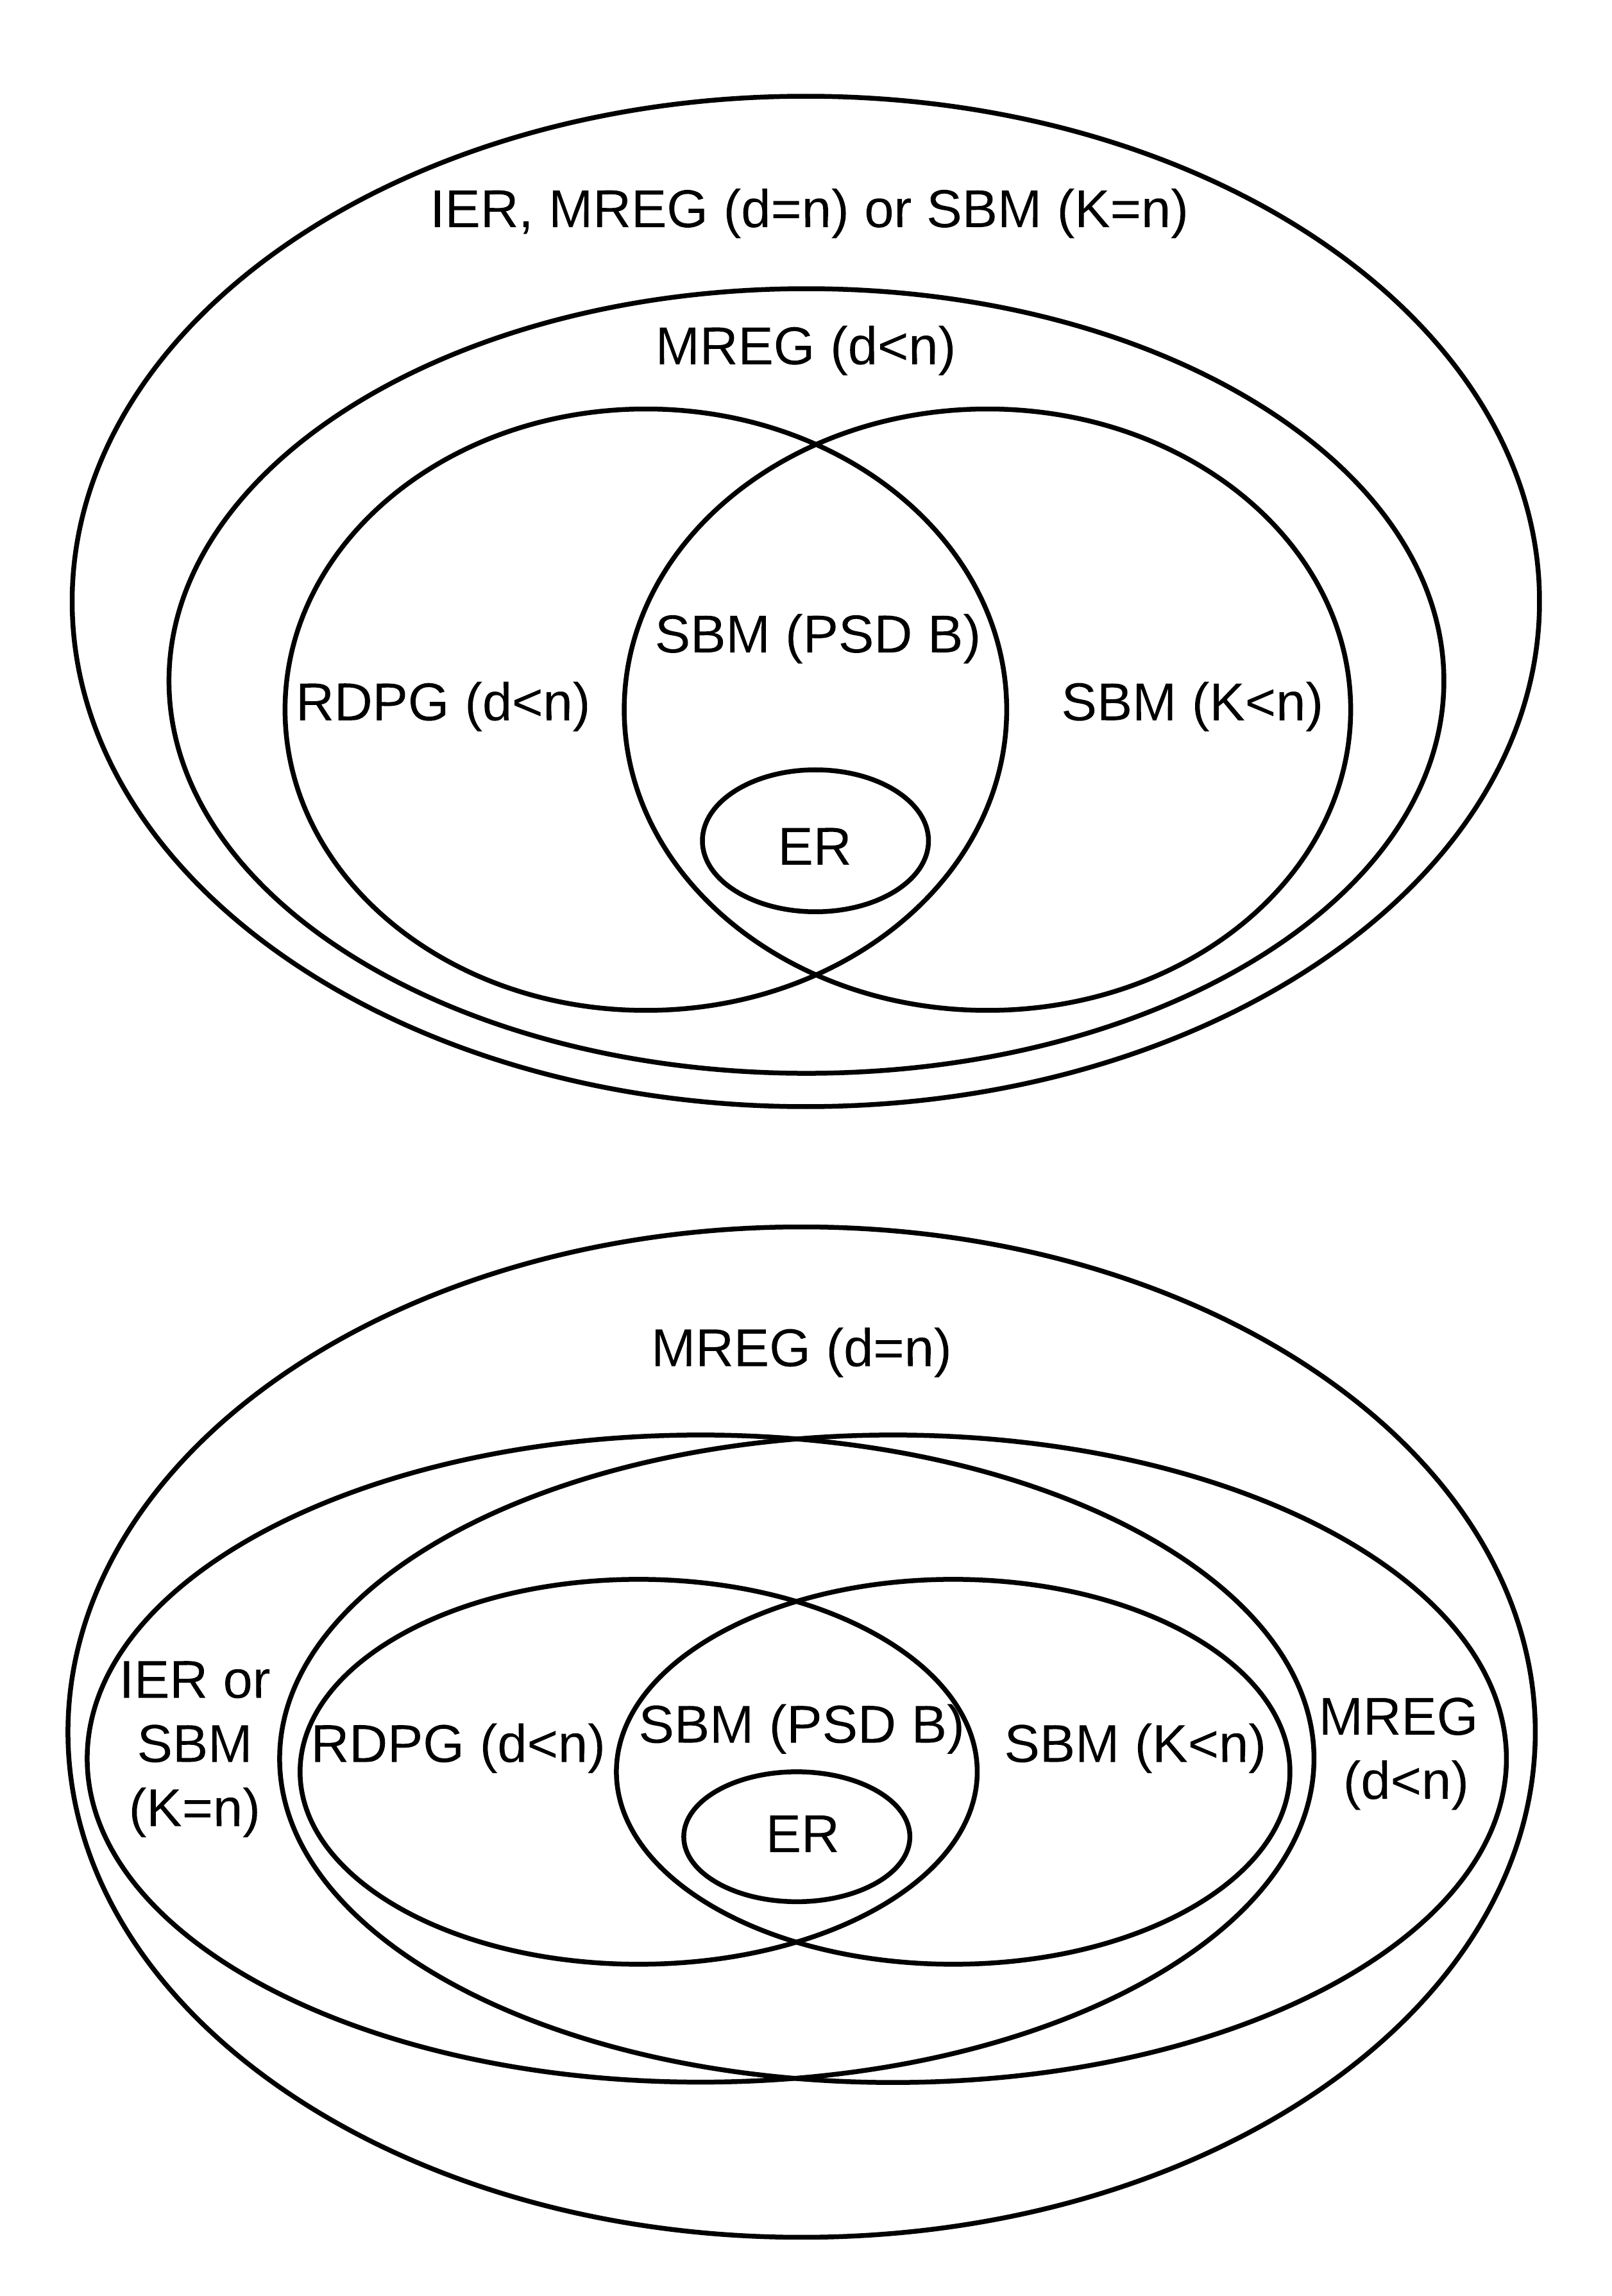
\includegraphics[scale=0.6,width=3.0in]{ven_diag.png}
	\caption{Relationship between random graph models on $1$ graph and multiple graphs. The top panel shows the relationship between random graph models on $1$ graph. The models considered are those conditioned on latent positions, that is $\tau$, $X$ and $\lambda$ in SBM, RDPG and MREG respectively are treated as parameters. ER is a $1$-block SBM. If a graph follows SBM with a positive semi-definite edge probability matrix, it also follows the RDPG model. Any  SBM and  RDPG graph can be represented by a $d$-dimensional MREG model with $d$ being less than or equal to the number of blocks or the dimension of RDPG. On one graph, inhomogeneous ER (IER), $n$-dimensional MREG and $n$-block SBM are equivalent. The bottom panel shows the relationship between random graph models on multiple graphs. The models considered are those conditioned on latent positions, and for ER, SBM and RDPG graphs are sampled i.i.d. with the same parameters. In this case, MREG has the flexibility to have $\lambda$ differ across graphs which leads to more generalized model for multiple graphs.}
	\label{fig:ven}
\end{figure}





\section{Methodology}
\subsection{Joint Embedding of Graphs}
The joint embedding method considers a collection of vertex-aligned graphs, and estimates a common embedding space across all graphs and a loading for each graph. Specifically, it simultaneously identifies a subspace spanned by a set of rank one symmetric matrices and projects each adjacency matrix $A_i$ into the subspace. The coefficients obtained by projecting $A_i$ are denoted by $\hat{\lambda}_i \in \mathbb{R}^d$, which is called the loading for graph $i$. To estimate rank one symmetric matrices and loadings for graphs, the algorithm minimizes the sum of squared Frobenius distances between adjacency matrices and their projections as described below.
\begin{definition} Joint Embedding of Graphs (JE). Given $m$ graphs $\{G_i \} _{i=1}^{m}$ with $A_i$ being the corresponding adjacency matrix, the $d$-dimensional joint embedding of graphs $\{G_i \} _{i=1}^{m}$ is given by
\begin{equation}\label{eq:1}
 (\hat{\lambda}_1,...,\hat{\lambda}_m,\hat{h}_1,...,\hat{h}_d) = \underset{\lambda_i,\|h_k\|=1}{\operatorname{argmin}} \sum\limits_{i=1}^{m} \| A_i- \sum\limits_{k=1}^{d} \lambda_{i}[k] h_k h_k^T \|  ^2.  
\end{equation}
Here, $\| \cdot \|$ denotes the Frobenius norm and $\lambda_{i}[k]$ is the $k$th entry of vector $\lambda_i$.
\end{definition}
To make sure that model is identifiable, we put an extra requirement on the norm of $h_k$. To ease our notation, we introduce two matrices $\Lambda \in \mathbb{R}^{m \times d}$ and $H\in \mathbb{R}^{n \times d}$, where $\lambda_i$ is the $i$th row of $\Lambda$ and $h_k$ is the $k$th row of $H$; that is, $\Lambda=[\lambda_1^T,...,\lambda_m^T]$ and $H=[h_1,...,h_d]$. We can rewrite equation~\eqref{eq:1} using $\Lambda$ and $H$ as
\begin{equation*}
(\hat{\Lambda},\hat{H}) = \underset{\Lambda,\|h_k\|=1}{\operatorname{argmin}} \sum\limits_{i=1}^{m} \| A_i- \sum\limits_{k=1}^{d} \Lambda_{ik} h_k h_k^T \|  ^2.  
\end{equation*}
 We denote the function on the left hand side of the equation by $f(\Lambda,H)$ which is explicitly a function of $\lambda_i$s and $h_k$s. There are several alternative ways to formulate the problem. If we convert $\lambda_i$ into a diagonal matrix $D_i \in \mathbb{R}^{d \times d}$ by putting entries of $\lambda_i$ on the diagonal of $D_i$, then solving equation \eqref{eq:1} is equivalent to solving
 \begin{equation*}
\begin{aligned}  
	& \underset{D_i,\|h_k\|=1}{\operatorname{argmin}} 
	& & \sum\limits_{i=1}^{m} \| A_i- H D_i H^T \|  ^2 \\
	& \text{ subject to} 
	& &  D_i \text{ being diagonal.}
\end{aligned}
\end{equation*}
We may also view \eqref{eq:1} as a tensor factorization problem. If $\{A_i\}_{i=1}^m$ are stacked in a 3-D array ${\bf A} \in \mathbb{R}^{m\times n \times n}$, then solving equation~\eqref{eq:1} is also equivalent to
\[  \underset{\Lambda,\|h_k\|=1}{\operatorname{argmin}}  \| {\bf A} - \sum\limits_{k=1}^{d} \Lambda_{*k} \otimes h_k \otimes h_k\|  ^2  \]
where $\otimes$ denotes the tensor product and $\Lambda_{*k}$ is the $k$th column of $\Lambda$. \\

\noindent The optimization problem in equation \eqref{eq:1} is similar to principal component analysis in the sense of minimizing squared reconstruction error to recover loadings and components \cite{jolliffe2002principal}. However, there are extra symmetries and rank constraints on the components. Similar optimization problems are also considered in the simultaneous diagonalization literature \cite{flury1986algorithm} \cite{ziehe2004fast}. The difference is that we are estimating an $n$-by-$d$ matrix $H$ by minimizing reconstruction error instead of finding a $n$-by-$n$ non-singular matrix by trying to simultaneously diagonalize all matrices. The problem in equation \eqref{eq:1} has considerably fewer parameters to optimize, which makes it more stable and applicable with $n$ being moderately large. In case of embedding only one graph, the joint embedding is equivalent to the Adjacency Spectral Embedding solved by singular value decomposition\cite{sussman2012consistent}. Next, we describe an algorithm to optimize the objective function $f(\Lambda,H)$.  

\subsection{Alternating Descent Algorithm}
\noindent The joint embedding of $\{G_i \} _{i=1}^{m}$ is estimated by solving the optimization problem in equation \eqref{eq:1}. There are a few methods proposed to solve similar problems. Carroll and Chang \cite{carroll1970analysis} propose to use an alternating minimization method that ignores symmetry. The hope is that the algorithm will converge to a symmetric solution itself due to symmetry in data. Gradient approaches have also been considered for similar problems \cite{tang2009clustering} \cite{kolda2015numerical}. We develop an alternating descent algorithm to minimize $f(\Lambda,H)$ that combines ideas from both approaches. The algorithm iteratively updates one of $\Lambda$ and $H$ while treating the other parameter as fixed. We will see that optimizing $\Lambda$ when fixing $H$ is easy, since it is essentially a least squares problem. However, optimizing $H$ when fixing $\Lambda$ is hard due to the fact that the problem is non-convex and there is no closed form solution available. In this case, we utilize gradient information and take an Armijo line search strategy to update $H$ \cite{nocedal2006numerical}. \\

\noindent Instead of optimizing all columns $\Lambda$ and $H$ simultaneously, we consider a greedy algorithm which solves the optimization problem by only considering one column of  $\Lambda$ and $H$ at a time. Specifically, the algorithm fixes all estimates for the first $k_0-1$ columns of $\Lambda$ and $H$ at iteration $k_0$, and then the objective function is minimized by searching through only the $k$th column of $\Lambda$ and $H$. That is,
\begin{align}(\hat{\Lambda}_{*k_0},\hat{h}_{k_0}) &= \underset{\Lambda_{*k_0},\|h_{k_0}\|=1}{\operatorname{argmin}} \nonumber\\ &\sum\limits_{i=1}^{m} \| A_i- \sum\limits_{k=1}^{k_0-1} \hat{\Lambda}_{ik} \hat{h}_{k} \hat{h}_{k}^T -\Lambda_{ik_0} h_{k_0} h_{k_0}^T\|  ^2.
\label{eq:2}
\end{align} 
Let $f(\Lambda_{*k_0},h_{k_0})$ denote the sum on the left hand side of the equation. To compute a $d$-dimensional joint embedding $(\hat{\Lambda},\hat{H})$, the algorithm iteratively solves the one dimensional optimization problem above by letting $k_0$ vary from $1$ to $d$. \\

\noindent There are a few advantages in iteratively solving one dimensional problems. First, there are fewer parameters to fit at each iteration, since the algorithm are only allowed to vary $\Lambda_{*k_0}$ and $h_{k_0}$ at iteration $k_0$. This makes initialization and optimization steps much easier compared to optimizing all columns of $H$ simultaneously. Second, it implicitly enforces an ordering on the columns of $H$. This ordering allows us to select the top few columns of $\Lambda$ and $H$ in cases where we want to perform model selection. Third, it allows incremental computation. If we compute $d$ and $d'$ dimensional joint embeddings, the first $\min(d,d')$ columns of $\hat{\Lambda}$ and $\hat{H}$ will be the same. Finally, based on numerical experiments, the difference between optimizing iteratively and optimizing all the parameters when $d$ is small is negligible; however, the iterative algorithm yields a slightly smaller objective function when $d$ is large. The disadvantage of optimizing each column separately is that the algorithm is more likely to end up at a local minimum when the objective function is structured not in favor of embedding iteratively. In practice, this problem can be mitigated by running the joint embedding algorithm several times with random initializations. \\ 

\noindent To find $\Lambda_{*k_0}$ and $h_{k_0}$ in equation\ref{eq:2}, the algorithm needs to evaluate two derivatives: $\frac{\partial f}{\partial h_{k_0}}$ and $\frac{\partial f}{\partial \Lambda_{i k_0}}$. Denote by $R_{ik_0}$ the residual matrix after iteration $k_0-1$ which is $A_i- \sum\limits_{k=1}^{k_0-1}\hat{\Lambda}_{ik} \hat{h}_{k} \hat{h}_{k}^T$. The gradient of the objective function with respect to $h_{k_0}$ is given by
\begin{equation} \label{eq:3}
\frac{\partial f}{\partial h_{k_0}} = -4\sum\limits_{i=1}^{m}  \Lambda_{ik_0} (R_{ik}-\Lambda_{ik_0} h_{k_0} h_{k_0}^T)  h_{k_0}.
\end{equation}
The derivative of the objective function with respect to $\Lambda_{i k_0}$ is given by
\[\frac{\partial f}{\partial \Lambda_{i k_0}}= -2 \langle R_{ik}-\Lambda_{ik_0} h_{k_0} h_{k_0}^T,h_{k_0} h_{k_0}^T\rangle.\]
Setting the derivative to $0$ yields
\begin{equation}  \label{eq:4}
\hat{\Lambda}_{i k_0} = \langle R_{ik}, h_{k_0} h_{k_0}^T \rangle,
\end{equation}
where $\langle \cdot , \cdot \rangle$ denotes the inner product. Algorithm 1 describes the general procedure to compute the $d$-dimensional joint embedding of graphs $\{G_i\}_{i=1}^m$. After the algorithm finishes, rows of $\hat{\Lambda}$ denoted by $\{\hat{\lambda}_i\}_{i=1}^m$ can be treated as estimates of $\{\lambda_i\}_{i=1}^m$ or features for graphs. Columns of $\hat{H}$ denoted by $\{\hat{h}_k\}_{k=1}^d$ are estimates of $\{h_k\}_{k=1}^d$ If a new graph $G$ is observed with adjacency matrix $A$, we can project $A$ into linear space spanned by $\{\hat{h}_k \hat{h}_k^T\}_{k=1}^{d}$ to obtain features for the graph. The optimization algorithm described above may not be the fastest approach to solving the problem; however, numerical optimization is not the focus of this paper. Based on results from numerical applications, our approach works well in estimating parameters and extracting features for subsequent statistical inference.
\begin{algorithm}
	\caption{Joint Embedding Algorithm}
	\begin{algorithmic}[1]
		\Procedure{Find joint embedding $\hat{\Lambda},\hat{H}$ of $\{A_i\}_{i=1}^m$}{}
		\State Set residuals: $R_{i1}=A_i$
		\For{$k=1:d$ }
		\State Initialize $h_k$ and $\Lambda_{*k}$ 
		\While{not convergent}
		\State Fixing $\Lambda_{*k}$, update $h_k$ by gradient descent \eqref{eq:3}
		\State Project $h_k$ back to the unit sphere
		\State Fixing $h_k$, update $\Lambda_{*k}$ by \eqref{eq:4}
		\State Compute objective $\sum\limits_{i=1}^{m} \| R_{ik}-  \Lambda_{ik} h_k h_k^T \|^2$
		\EndWhile
		\State Update residuals: $R_{i(k+1)}=R_{ik}- \Lambda_{ik} h_kh_k^T$
		\EndFor
		\State Output $\hat{\Lambda}=[\Lambda_{*1},...,\Lambda_{*d}]$ and $\hat{H}=[h_1,...,h_d]$
		\EndProcedure
	\end{algorithmic}
\end{algorithm}



\subsection{Variations}
The joint embedding algorithm described above can be modified to accommodate several settings. \\
\textbf{Variation 1.} When all graphs come from the same distribution, we can force estimated loadings $\hat{\lambda}_i$ to be equal across all graphs. This is useful when the primary inference task is to extract features for vertices. Since all graphs share the same loadings, with slightly abusing notations, let $\Lambda$ be a vector in $\mathbb{R}^d$ and the optimization problem becomes
\[ (\hat{\Lambda},\hat{H}) = \underset{\Lambda,\|h_k\|=1}{\operatorname{argmin}} \sum\limits_{i=1}^{m} \| A_i- \sum\limits_{k=1}^{d} \Lambda_{k} h_k h_k^T \|  ^2.  \] 
In this case, the optimization problem can be solved exactly by finding the singular value decomposition of the average adjacency matrix $\frac{1}{m}\sum\limits_{i=1}^{m}A_i$. \\
\textbf{Variation 2.} When there is a discrete label $y_i \in \mathbb{Y}$ associated with $G_i$ available, we may require all loadings $\hat{\lambda}_i$ to be equal within class. If we let $\Lambda \in \mathbb{R}^{|\mathbb{Y}| \times d}$, the optimization problem becomes
\[ (\hat{\Lambda},\hat{H}) = \underset{\Lambda,\|h_k\|=1}{\operatorname{argmin}} \sum\limits_{i=1}^{m} \| A_i- \sum\limits_{k=1}^{d} \Lambda_{y_i k} h_k h_k ^T \|  ^2.  \] 
In this case, when updating $\Lambda$ as in equation \ref{eq:4}, the algorithm should average $\Lambda_{y_i k}$ within the same class. \\
\textbf{Variation 3.} In some applications, we may require all $\Lambda_{ik}$ to be greater than $0$, as in non-negative matrix factorization. One advantage of this constraint is that graph $G_i$ may be automatically clustered  based on the largest entry of $\hat{\lambda}_{i}$. In this case, the optimization problem is
\[ (\hat{\Lambda},\hat{H}) = \underset{\Lambda \geq 0,\|h_k\|=1}{\operatorname{argmin}} \sum\limits_{i=1}^{m} \| A_i- \sum\limits_{k=1}^{d} \Lambda_{ik} h_k h_k ^T \|  ^2.  \] 
To guarantee nonnegativity, the algorithm should use nonnegative least squares in updating $\Lambda$ \cite{kim2008nonnegative}. Next, we discuss some theoretical properties of joint embedding when treated as a parameter estimation procedure for the MREG model.

\section{Theory}
In this section, we consider a simple setting where graphs follow a $1$-dimensional MREG model, that is $\{(\lambda_i,A_i)\} _{i=1}^m \sim MREG(F,h_1)$. Under this MREG model, we can understand joint embedding of graphs as estimators for parameters of the model. Specifically, $\hat{\lambda}_i$ and $\hat{h}_1$ are estimates of $\lambda_i$ and $h$. We prove the following two theorems concerning the asymptotic behavior of estimator $\hat{h}_1$ produced by joint embedding. Let $\hat{h}_1^m$ denote the estimates based on $m$ graphs and define functions $\rho$, $D_m$ and $D$ as below: 
\[ \rho(A_i,h)= \|A_i- \langle A_i,h h^T \rangle h h^T\|^2, \]
\[ D_m(h,h_1) =\frac{1}{m}\sum_{i=1}^{m} \rho(A_i,h), \]
\[ D(h,h_1) = E(\rho(A_i,h)). \]
By equation \eqref{eq:1}, we have
\begin{align*} 
\hat{h}_1^m = \underset{\|h\| =1}{\operatorname{argmin}} \text{ }   \underset{\lambda_i}{\operatorname{argmin}} \sum_{i=1}^{m} \|A_i - \lambda_i h h^T\| .
\end{align*}
By equation \eqref{eq:4}, we have 
\[\langle A_i,hh^T \rangle=\underset{\lambda_i}{\operatorname{argmin}} \sum_{i=1}^{m} \|A_i - \lambda_i h h^T\|.\]
Therefore,
\[\hat{h}_1^m = \underset{\|h\| =1}{\operatorname{argmin}} \text{ } D_m(h,h_1). \]
The first theorem states that $\hat{h}_1^m$  converges almost surely to the global minimum of $D(h,h_1)$, given that the global minimum is unique.
\begin{theorem}
\label{thm:1}
If $D(h,h_1)$ has a unique global minimum at $h'$, then $\hat{h}_1^m$ converges almost surely to $h'$ as $m$ goes to infinity. That is, 
\[ \hat{h}_1^m \overset{a.s.}{\rightarrow} h'. \]
\end{theorem}

\noindent In Theorem \ref{thm:1}, we require $h'$ to be the unique global minimizer of $D(h,h_1)$. However, the global minimizer is definitely not unique due to the symmetry up to sign flip of $h$, that is $D(h,h_1)=D(-h,h_1)$ for any $h$. This problem can be addressed by forcing an orientation of $\hat{h}_1^m$ or stating that the convergence is up to a sign flip. It is also possible that there are multiple global minimizers of $D(h,h_1)$ which are not sign flips of each other. In this case, Theorem \ref{thm:1} does not apply. We are currently only certain that when all graphs are from the Erdos-Renyi random graph model, the global minimizer is unique up to a sign flip. The next theorem concerns the asymptotic bias of $\hat{h}_1^m$. 

\begin{theorem}
\label{thm:2}
If $h'$ is a minimizer of $D(h,h_1)$, then 
\[\|h'-h_1\| \leq \frac{2 E(\lambda_i)}{E(\lambda_i^2)(h_1^T h')^2}. \]
\end{theorem}

\noindent	To see an application of Theorem \ref{thm:2}, we consider the case in which all graphs are Erdos-Renyi graphs with $100$ vertices and edge probability of $0.5$. Under this setting, Theorem \ref{thm:2} implies  $\|h'-h_1\| \in [0,0.04] \cup [1.28,1.52]$. The second interval is disturbing. It is due to the fact that when $h_1^T h'$ is small, the bound is useless. We provide some insights as to why the second interval is there and how we can get rid of it with additional assumptions. In the proof of Theorem \ref{thm:2}, we show that the global optimizer $h'$ satisfies
\[h'= \underset{\|h\| =1}{\operatorname{argmax}} \text{ } E(\langle A_i,h h^T \rangle ^2). \]
If we take a closer look at $E(\langle A_i,h h^T \rangle ^2)$, we see
\begin{align*}
	E(\langle A_i,h h^T \rangle ^2) &= E(\langle P_i,h h^T \rangle ^2)+E(\langle A_i-P_i,h h^T \rangle ^2) \\
	&=E(\lambda_i^2)(h_1^T h)^4+E((h^T (A_i-P_i)h) ^2).
\end{align*}
Therefore, 
\[h'= \underset{\|h\| =1}{\operatorname{argmax}} \text{ } E(\lambda_i^2)(h_1^T h)^4+E((h^T (A_i-P_i)h) ^2) .\]
We can see that $E(\lambda_i^2)(h_1^T h)^4$ is maximized when $h=h_1$; however, the noise term $E((h^T (A_i-P_i)h) ^2)$ is generally not maximized at $h=h_1$. If we assume $n$ is large, we can apply a concentration inequality to $(h^T (A_i-P_i)h) ^2$ and have an upper bound on $E((h^T (A_i-P_i)h) ^2)$. If we further assume $A_i$ is not too sparse, that is $E(\lambda_i^2)$ grows with $n$ fast enough, then the sum of these two terms is dominated by the first term. This provides a way to have a lower bound on $h_1^T h'$. We may then replace the denominator of the bound in Theorem \ref{thm:2} by the lower bound. In general, if $n$ is small, the noise term may cause $h'$ to differ from $h_1$ by a significant amount. In this paper, we focus on the case that $n$ is fixed. The case that $n$ goes to infinity for random dot product graphs is considered in \cite{athreya2013limit}.\\


\noindent The two theorems above concern only the estimation of $h_1$, but not $\lambda_i$. Based on equation \eqref{eq:4}, we estimate $\lambda_i$ by
\[\hat{\lambda}_i^m= \langle A_i,\hat{h}_1^m \hat{h}_1^{m T} \rangle. \]
If $n$ is fixed, it is impossible to prove any consistency result on estimation of $\lambda_i$ due to the fact we observe only one finite graph $A_i$ associated with $\lambda_i$. When $m$ goes to infinity, we can apply Theorem \ref{thm:1},
\[\hat{\lambda}_i^m = \langle A_i,\hat{h}_1^m \hat{h}_1^{mT} \rangle \overset{a.s.}{\rightarrow} \langle A_i,h' h'^T \rangle = h'^T A_i h'.\]
Then, applying the bound on $\|h'-h_1\|$ derived in Theorem \ref{thm:2} and utilizing the fact that $h^T A_i h$ is continuous in $h$, we can have an upper bound on $|\hat{\lambda}_i^m - h_1^T A_i h_1|$. When $A_i$ is large, $h_1^T A_i h_1$ is concentrated around $\lambda_i$ with high probability. In the next section, we demonstrate properties and utilities of the joint embedding algorithm. 

\section{Experiments}
Before going into details of our experiments, we want to discuss how to select the dimensionality $d$ of the joint embedding. Estimating $d$ is an important model selection question that has been studied for years under various settings \cite{kohavi1995study}. It is not the focus of this paper, but we still face this decision in numerical experiments. In the simulation experiments of this section, we assume $d$ is known to us and simply set the dimensionality estimate $\hat{d}$ equal to $d$. In the real data experiment, we recommend two approaches to determine $\hat{d}$. Both approaches require we first run the $d'$-dimensional joint embedding algorithm, where $d'$ is sufficiently large and we are confident that $d$ is less than $d'$. We then plot the objective function versus dimension, and determine $\hat{d}$ to be where the objective starts to flatten out. Alternatively, we can plot $\{\hat{\Lambda}_{ik}\}_{i=1}^m$ for $k=1,...,d'$, and select $\hat{d}$ when the loadings start to look like noise with $0$ mean. These two approaches should yield a similar dimensionality estimate of $\hat{d}$. 

\subsection{Simulation Experiment 1: Joint Embedding Under a Simple Model}
\noindent We present a simple numerical example to demonstrate some properties
of our joint embedding procedure as the number of graphs grows. We repeatedly generate graphs with $5$ vertices from $1$-dimensional MREG where $\lambda_i \sim Unif(1,2)$ and $h_1=[0.1,0.2,0.3,0.4,0.5]^T/0.74$. We keep doubling the number of graphs $m$ from $2^4$ to $2^{16}$. At each value of $m$, we compute the $1$-dimensional joint embedding of $m$ graphs. Let the estimated parameters based on $m$ graphs be denoted by $\hat{\lambda}_i^m$ and $\hat{h}_1^m$. Two quantities based on $\hat{h}_1^m$ are calculated. The first is the norm difference between the current $h_1$ estimates and the previous estimates, namely $\|\hat{h}_1^m-\hat{h}_1^{m/2}\|$. This provides numerical evidence for the convergence of our principled estimation procedure. The second quantity is $\|\hat{h}^m_1-h_1\|$. This investigates whether $\hat{h}_1$ is an unbiased estimator for $h_1$. The procedure described above is repeated $100$ times. Figure \ref{fig:db} presents the result. \\

\begin{figure}[!htbp]
	\centering
	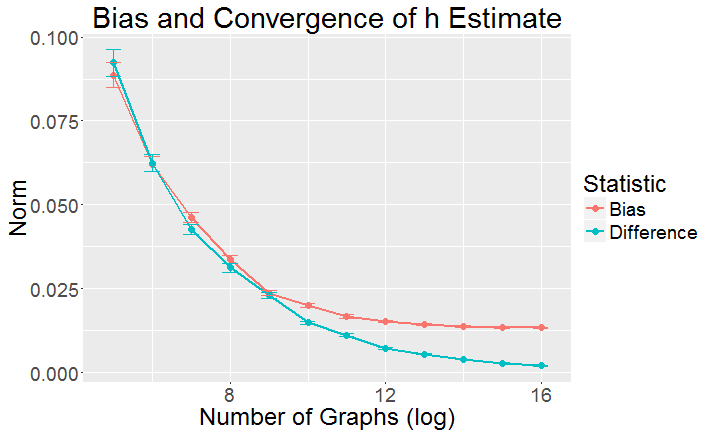
\includegraphics[scale=0.6,width=3.0in]{biasandconv.png}
	\caption{Mean bias ($\|\hat{h}^m_1-h_1\|$) and mean difference between estimates ($\|\hat{h}_1^m-\hat{h}_1^{m/2}\|$) across $100$ simulations are shown. The standard errors across $100$ simulations are also given by error bars. The graphs are generated from a $1$-dimensional MREG model as described in section 5.1. Bias stops decreasing at approximately $0.015$, and difference converges to $0$.}
	\label{fig:db}
\end{figure}

\noindent From the plot, we can see that the norm difference converges to $0$ as $m$ increases. This suggests the convergence of $\hat{h}_1^m$. Secondly, we notice that the bias $\|\hat{h}^m_1-h_1\|$ does not converge to $0$; instead, it stops decreasing at around $0.015$. This suggests that $\hat{h}_1$ is an asymptotically biased estimator for $h_1$. The $\hat{h}_1^m$ with $m=2^{16}$ is $[0.083,0.186, 0.296, 0.406, 0.503]^T/0.74$. Compared to $h_1$, there are negative biases for small entries of $h_1$, and positive biases for large entries of $h_1$. Actually, this is as to be expected: when there are infinitely many nuisance parameters present, Neyman and Scott demonstrate that maximum likelihood estimator is inconsistent \cite{neyman1948consistent}. In our case, there are infinitely many $\lambda_i$ as $m$ grows; therefore, we do not expect joint embedding to provide a consistent estimate of $h_1$. \\

\noindent In applications such as clustering or classifying multiple graphs, we may be not interested in $\hat{h}_1$. We are more interested in the $\hat{\lambda}_i$, which provide information specifically about the graphs $G_i$. Here, we consider two approaches to estimate $\lambda_i$. The first approach is estimating $\lambda_i$ through joint embedding, that is
\[ \hat{\lambda}_i = \langle A_i,  \hat{h}^m_1 \hat{h}^{m T}_1 \rangle. \]
The second approach estimates $\lambda_i$ by forcing $\hat{h}_1$ equal to $h_1$, that is 
\[ \hat{\lambda}_i = \langle A_i,  h_1 h_1^T \rangle. \]
$\hat{\lambda}_i$ calculated this way can be thought of as the 'oracle' estimate, since it assumes $h_1$ is known. For each value of $m$, Figure \ref{fig:ld} shows the differences in estimates provided by two approaches. Not surprisingly, the differences are small due to the fact that $\hat{h}_1^m$ and $h_1$ are close.
\begin{figure}[!htbp]
	\centering
	\includegraphics[scale=0.6,width=3.0in]{lambda_differ.png}
	\caption{Distribution of differences between $\hat{\lambda}_i$ estimated using $\hat{h}_1^m$ and $h_1$. The graphs are generated from a $1$-dimensional MREG model as described in section 5.1. The differences are small due to the fact that $\hat{h}_1^m$ and $h_1$ are close.}
	\label{fig:ld}
\end{figure}

\subsection{Simulation Experiment 2: Joint Embedding to Classify Graphs}
In this experiment, we consider the inference task of classifying graphs.  We have $m$ pairs $\{(A_i,Y_i)\}_{i=1}^{m}$ of observations. Each pair consists of an adjacency matrix $A_i \in \{0,1\}^{n \times n}$ and a label $Y_i \in [K]$. Furthermore, all pairs are assumed to be independent and identically distributed according to an unknown distribution $\mathbb{F}_{A,Y}$, that is
\[(A_1,Y_1),(A_2,Y_2),...,(A_m,Y_m) \overset{i.i.d.}{\sim} \mathbb{F}_{A,Y}. \] 
The goal is to find a classifier $g$ which is a function $g:\{0,1\}^{n \times n} \rightarrow [K]$ that has a small classification error $L_g=P(g(A)\neq Y)$. \\ 

\noindent We consider a binary classification problem where $Y$ takes value $1$ or $2$. We independently generate $200$ graphs with 100 vertices. The graphs are sampled from a $2$-dimensional MREG model. Let $h_1$ and $h_2$ be two vectors in $\mathbb{R}^{100}$, and \[h_1=[0.1,...,0.1]^T \text{ , and } h_2=[-0.1,...,-0.1,0.1,...,0.1]^T. \] 
Here, $h_2$ has $-0.1$ as its first $50$ entries and $0.1$ as its last $50$ entries. We generate graphs according to the MREG model, 
\begin{equation}
A_i \sim MREG(F,h_1,h_2).
\label{eq:simu}
\end{equation}
Here, $F$ is a mixture of two point masses with equal probability, 
\[ F = \frac{1}{2}\mathbb{I} \{\lambda=[25,5]\} + \frac{1}{2}\mathbb{I} \{\lambda=[22.5,2.5]\}.\]
We let the class label $Y_i$ indicate which point mass $\lambda_i$ is sampled from. In terms of SBM, this graph generation scheme is equivalent to 
\[ A_i|Y_i=1 \sim  SBM((1,...,1,2,...,2),\begin{bmatrix} 0.3 & 0.2 \\ 0.2 & 0.3 \\ \end{bmatrix})  \]
\[ A_i|Y_i=2 \sim  SBM((1,...,1,2,...,2),\begin{bmatrix} 0.25 & 0.2 \\ 0.2 & 0.25 \\ \end{bmatrix}).\]

\noindent To classify graphs, we first jointly embed $200$ graphs. The first two dimensional loadings are shown in Figure \ref{fig:load}. We can see two classes are clearly separated after being jointly embedded.
\begin{figure}[!htbp]
	\centering
	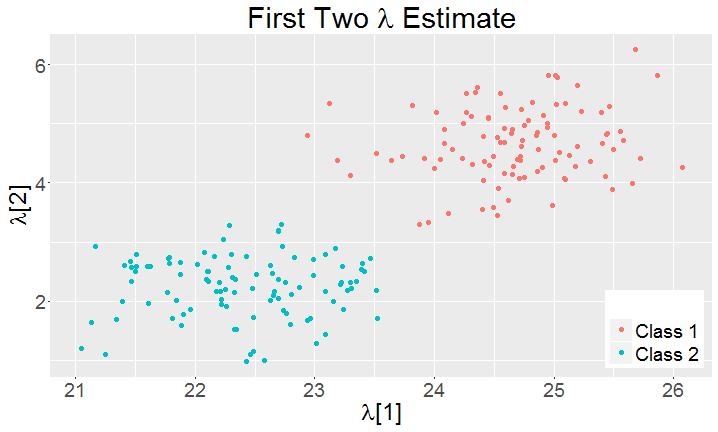
\includegraphics[scale=0.6,width=3.0in]{JE_200.png}
	\caption{Scatter plot of loadings computed by jointly embedding $200$ graphs. The graphs are generated from a $2$-dimensional MREG model as described in equation \ref{eq:simu}. The loadings of two classes are clearly separated after being jointly embedded. }
	\label{fig:load}
\end{figure}
Then, a $1$-nearest neighbor classifier is constructed based on loadings $\{\hat{\lambda}_i\}_{i=1}^m$. The $1$-NN classification error with $200$ graphs is $0$. \\
\\
\noindent We compare classification performance using joint embedding and Laplacian Eigenmap \cite{belkin2003laplacian}. For Laplacian Eigenmap, we first embed each normalized Laplacian matrix and then compute the Procrustes distance between embeddings. We also apply a $1$-NN rule to classify graphs. We let the number of graphs $m$ increase from $4$ to $200$. For each value of $m$, we repeat the simulation $100$ times. The result is shown in Figure \ref{fig:acc}. We see joint embedding takes advantage of increasing sample size and dominates the Laplacian Eigenmap at all values of $m$. 
\begin{figure}[!htbp]
	\centering
	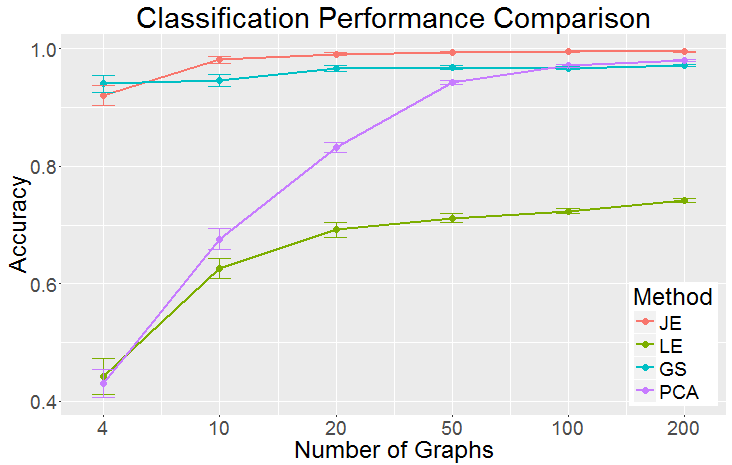
\includegraphics[scale=0.6,width=3.0in]{leig_je_acc.png}
	\caption{Mean classification accuracy of joint embedding (JE) and Laplacian Eigenmap (LE) with their standard errors are shown. The graphs are generated from a $2$-dimensional MREG model as described in equation \ref{eq:simu}. The graphs are first embedded using two approaches, and then apply a $1$-NN to the embeddings. For each value of $m$, the simulation is repeated $100$ times. Joint embedding takes advantage of increasing sample size and has nearly perfect classification performance when given more than $100$ graphs. Joint embedding dominates Laplacian eigenmap at all values of $m$.}
	\label{fig:acc}
\end{figure} 

\subsection{Real Data Experiment: Predict Composite Creativity Index}
In this experiment, we study predicting individual composite creativity index (CCI) through brain connectomes obtained by Multimodal Magnetic Resonance Imaging \cite{koutra2013d}. Neuroimaging and creativity have been jointly investigated previously. Most studies utilize a statistical testing method and find CCI significantly related or inversely related to the activity of some regions of the brain \cite{arden2010neuroimaging}. We embrace a different approach by directly building a prediction model for CCI. First, we jointly embed brain graphs of all subjects. Then, we construct a linear regression model by treating the estimated loadings as explanatory variables and CCI as the response variable. \\

\noindent In total, $113$ healthy, young adult subjects were scanned using a Siemens TrioTim scanner. 3D-MPRAGE and DTI in $35$ directions of the subjects were acquired \cite{brant1992mp}. The images were then registered by Desikan-Killiany Atlas \cite{desikan2006automated}, and a graph of $70$ vertices is constructed. The process of transforming MRI to graphs was completed by NeuroData's MRI Graphs pipeline\cite{kiar2016ndmgcode}. The graphs derived have weighted edges. One example of a graph is shown in the top panel of Figure \ref{fig:cci1}. For each subject, a divergent thinking measure was scored by independent judges using the Consensual Assessment Technique \cite{amabile1983social}, from which the CCI is derived. To predict the CCI, we first jointly embed $113$ graphs with $d=10$, and then fit a linear model by regressing CCI on $\hat{\lambda}_i$, that is
\[CCI_i \sim \beta_0+\lambda_i^T\beta + \epsilon_i. \]
Next, we assess the statistical significance of this model by comparing to the null model with only the intercept. \\

\noindent If only $\hat{\lambda}_i[1]$ is used as the explanatory variable, the top panel of Figure \ref{fig:cci} shows the result. We can see a significant positive linear relationship between CCI and the first dimensional loadings. The first dimensional loadings generally capture the overall connectivity of graphs. In our case, the correlation between the first dimensional loadings and the sum of edge weights is around $0.98$. This model implies that the individual tends to be more creative when there is more brain connectivity. The R-square of this model is $0.07248$, and the model is statistically significantly better when compared to the null model with a p-value $0.0039$, according to the F-test. If we fit CCI to all the $10$ dimensional loadings, a summary of the linear model is provided in the appendix and a scatter plot of fitted CCI versus true CCI is provided in the bottom panel of Figure \ref{fig:cci}. The R-square is $0.2325$ and the model is statistically significantly better than the null model with a p-value $0.0018$ according to the F-test. It is also significantly better than the model with only $\hat{\lambda}_i[1]$. Although there is still a positive relationship between CCI and the first dimensional loadings, it is no longer significant due to the inclusion of more explanatory variables. In this model, there is a significant negative relationship between CCI and $\hat{\lambda}_i[6]$ based on the t-test. The scatter plot of CCI against $\hat{\lambda}_i[6]$ is given in the middle panel of Figure \ref{fig:cci}. We look into the rank one matrix $\hat{h}_6^T\hat{h}_6$, which is shown in the bottom panel of figure \ref{fig:cci1}. It has positive connectivity within each hemisphere of the brain, but negative connectivity across hemispheres. This suggests that compared to within-hemisphere connectivity, across-hemisphere connectivity tends to have a more positive impact on human creativity. 

\begin{figure}[!htbp]
	\centering
	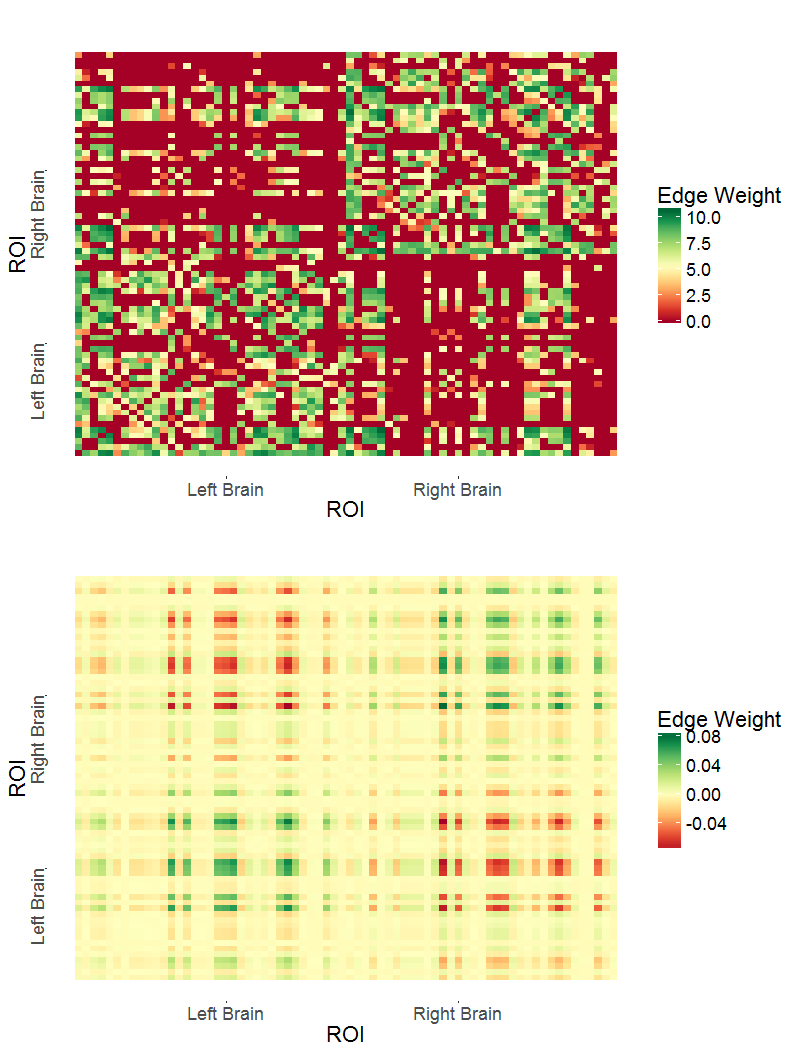
\includegraphics[width=3.0in]{cci_data.png}
	\caption{The top panel shows the graph derived from a typical subject. There is much more neural connectivity within each hemisphere. The bottom panel shows the rank one matrix $\hat{h}_6^T\hat{h}_6$, which has positive  connectivity within each hemisphere, but negative  connectivity across hemispheres.  }
	\label{fig:cci1}
\end{figure} 

\begin{figure}[!htbp]
	\centering
	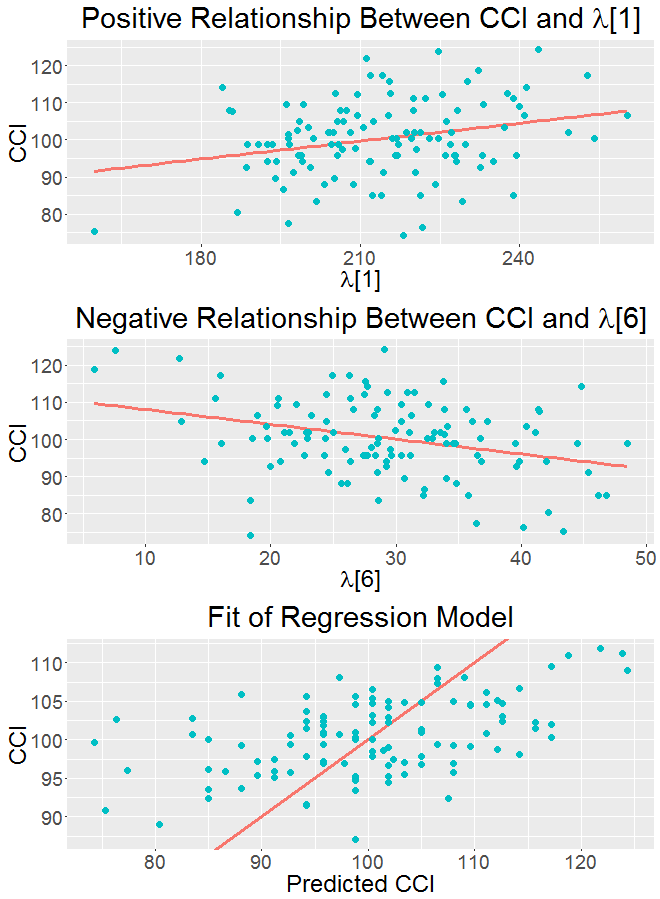
\includegraphics[scale=0.6,width=3.0in]{cci.png}
	\caption{The top panel shows the scatter plot of CCI against $\hat{\lambda}_i[1]$ with the regression line. There is a positive relationship between CCI and first dimensional loadings. The middle panel shows the scatter plot of CCI against $\hat{\lambda}_i[6]$ with regression line. There is a negative relationship between CCI and sixth dimensional loadings. The bottom panel shows the predicted CCI versus true CCI with the identity line.}
	\label{fig:cci}
\end{figure}


\section{conclusion}
In summary, we developed a joint embedding method that can simultaneously embed multiple graphs into low dimensional space. Joint embedding can be used to estimate features for inference problems on multiple vertex matched graphs. Learning on multiple graphs has significant applications in diverse fields and our results have both theoretical and practical implications for the problem. As the real data experiment illustrates, joint embedding is a practically viable inference procedure. We also propose a Multiple Random Eigen Graphs model. It can be understood as a generalization of the Random Dot Product Graph model or the Stochastic Block Model for multiple random graphs. We analyzed the performance of joint embedding on this model under simple settings. We show that the joint embedding method provides estimates with bounded error. Our approach is intimately related to other matrix and tensor factorization approaches such as singular value decomposition and CP decomposition. Indeed, joint embedding and these algorithms all try to estimate a low dimensional representation of high dimensional objects. We are currently the utility of investigating the joint embedding with more or less regularizations on parameters and under different set ups. We are optimistic that our method provides a viable tool for analyzing multiple graphs and can contribute to a deeper understanding of the joint structure of networks.


%\appendix
\section*{Appendix A}

\begin{proof} [Proof of Theorem 2.1]
 Let $P_i$ be the edge probability matrix of graph $i$ which is a real symmetric matrix with $\frac{n(n+1)}{2}$ free entries. It lies in a linear space with dimensionality $\frac{n(n+1)}{2}$. As a consequence, if there exists $\frac{n(n+1)}{2}$ linear independent rank one symmetric matrices, they form a basis for this space. One can check that the rank one symmetric matrices generated by vectors $\{e_i\}_{i=1}^{n} \cup \{e_i+e_j\}_{i<j}$ are linearly independent, where $\{e_i\}_{i=1}^{n}$ is the standard basis for $n$-dimensional Euclidean space. Let $\{e_i\}_{i=1}^{n} \cup \{\frac{e_i+e_j}{\sqrt{2}}\}_{i<j}$ be the $h$s in MREG model. The discussion above implies $P_i$ can be represented as a linear combination rank one matrices generated by $h$s. This concludes that $\frac{n(n+1)}{2}$-dimensional MREG can represent any set of edge independent graphs. 
\end{proof}

\begin{proof} [Proof of Theorem 4.1]
First,  we show that $|D_n(h,h_1)-D(h,h_1)|$ converges uniformly to $0$.
We notice three facts:
\begin{itemize}
	\item[(1)] the set $\{h: \|h\|=1\}$ is compact;
	\item[(2)] for all $h$, the function $\rho(\cdot,h)$ is continuous
	\item[(3)] for all $h$, the function $\rho(\cdot,h)$ is bounded by $n^2$.
\end{itemize}
Therefore, by the uniform law of large numbers \cite{jennrich1969asymptotic}, we have
\[\underset{h}{\sup}|D_m(h,h_1)-D(h,h_1)|\overset{a.s.}{\rightarrow} 0.\]
To prove the claim of the theorem, we use a technique similar to that employed by Bickel and Doksum \cite{bickel2015mathematical}. By definition, we have $D_m(\hat{h}_1^m,h)  \leq D_m(h',h)$ and $D(h',h) \leq D(\hat{h}_1^m,h)$. From these two inequalities we obtain
\begin{align*}
D_m(h',h)-D(h',h) &\geq D_m(\hat{h}_1^m,h)-D(h',h) \\
&\geq D_m(\hat{h}_1^m,h)-D(\hat{h}_1^m,h) .
\end{align*}
Therefore, 
\begin{align*}
|D_m(\hat{h}_1^m,h)-D(h',h)|  \leq  \max(&|D_m(h',h)-D(h',h)|,\\
& |D_m(\hat{h}_1^m,h)-D(\hat{h}_1^m,h)|).
\end{align*}
This implies 
\[ |D_m(\hat{h}_1^m,h)-D(h',h)| \leq \underset{h}{\sup}|D_m(h,h_1)-D(h,h_1)|. \]
Hence, $|D_m(\hat{h}_1^m,h)-D(h',h)|$ must converge almost surely to $0$, that is
\[|D_m(\hat{h}_1^m,h)-D(h',h)|\overset{a.s.}{\rightarrow} 0 .\]
 If $\hat{h}_1^m$ does not converge almost surely to $h'$, then  $\|\hat{h}_1^m-h'\|\geq \epsilon$ for some $\epsilon$ and infinitely many values of $m$. Since $h'$ is the unique global minimum, $|D(\hat{h}_1^m,h)-D(h',h)| > \epsilon' $ for infinitely many values of $m$ and some $\epsilon' $. This contradicts with the previous equation. Therefore, $\hat{h}_1^m$ must converge almost surely to $h'$.
\end{proof}


\begin{proof} [Proof of Theorem 4.2]
The first part of proof involves showing that $h'$ is the eigenvector corresponding to the largest eigenvalue of $E(\langle A_{i},h' h'^T \rangle A_{i})$. Then, we show $E(\langle A_{i},h' h'^T \rangle A_{i})$ is close to a properly scaled $E(P_i)$. To conclude, we apply the Davis-Kahan theorem to the top eigenvector of both matrices to obtain the desired result. First, we notice that
	\begin{align*}
	\underset{\|h\| =1}{\operatorname{min}}D(h,h_1) &=\underset{\|h\| =1}{\operatorname{min}}E(\|A_i- \langle A_i,h h^T \rangle h h^T\|^2) \\
	&=\underset{\|h\| =1}{\operatorname{min}}E(\langle A_i,A_i \rangle- \langle A_i,h h^T \rangle ^2) \\
	&=E(\langle A_i,A_i \rangle)-\underset{\|h\| =1}{\operatorname{max}}E( \langle A_i,h h^T \rangle ^2).
	\end{align*}
	Therefore, 
	\begin{equation} \label{eq:5}
	h'= \underset{\|h\| =1}{\operatorname{argmin}} \text{ }D(h,h_1)=\underset{\|h\| =1}{\operatorname{argmax}} \text{ } E(\langle A_i,h h^T \rangle ^2) .
	\end{equation}
	Taking the derivative of $E( \langle A_i,h h^T \rangle ^2)+ c(h^Th-1)$ with respect to $h$, we have 
	\begin{align*}
	\frac{\partial E( \langle A_i,h h^T \rangle ^2)+ c(h^Th-1) }{\partial h} & =  E(\frac{\partial  \langle A_i,h h^T \rangle ^2}{\partial h}) +2ch \\
	&=4 E( \langle A_i,h h^T \rangle A_i)h +2ch .
	\end{align*}
	Setting this expression to $0$ yields,
	\begin{align*} 
	E( \langle A_i,h' h'^T \rangle A_i)h' & = -\frac{1}{2}ch' .
	\end{align*}
	Using the fact that $\|h'\|=1$, we can solve for $c$:
	\[c = -2 h'^T E( \langle A_i,h' h'^T \rangle A_i)h' = -2 E( \langle A_i,h' h'^T \rangle^2) .\]
	Then, substituting for $c$, we obtain
	\begin{equation}
	E( \langle A_i,h' h'^T \rangle A_i)h'=E( \langle A_i,h' h'^T \rangle^2)h'.
	\end{equation}
	Therefore, we see that $h'$ is an eigenvector of $E(\langle A_{i},h' h'^T \rangle A_{i})$ and the corresponding eigenvalue is $E(\langle A_{i},h' h'^T \rangle ^2)$. Furthermore, $E(\langle A_{i},h' h'^T \rangle ^2)$ must be the eigenvalue with the largest magnitude. For if not, then there exists an $h''$ with norm $1$ such that
	\begin{align*}  | h''^T E(\langle A_{i},h' h'^T \rangle A_{i}) h''| &= |E(\langle A_{i},h' h'^T \rangle \langle A_{i},h'' h''^T \rangle)| \\
	&> E(\langle A_{i},h' h'^T \rangle ^2);
	\end{align*}
	however, by Cauchy-Schwarz inequality we must have
	\begin{align*} E(\langle A_{i},h'' h''^T \rangle^2)  E(\langle A_{i},h' h'^T \rangle^2) &> \\
	&|E(\langle A_{i},h' h'^T \rangle \langle A_{i},h'' h''^T \rangle)|^2,
	\end{align*}
	implying $E(\langle A_{i},h'' h''^T \rangle^2) > E(\langle A_{i},h' h'^T \rangle^2)$, which contradicts equation \eqref{eq:5}. Thus we conclude that $h'$ is the eigenvector corresponding to the largest eigenvalue of $E(\langle A_{i},h' h'^T \rangle A_{i})$. Next, we compute $E(\langle A_{i},h' h'^T \rangle A_{i})$.
	\begin{align*}
	&E(\langle A_{i},h' h'^T \rangle A_{i}|P_i)    \\
	&=E( \langle A_{i}-P_i,h' h'^T \rangle (A_{i}-P_i)|P_i)\\
	&\qquad {}+E(\langle A_{i}-P_i,h' h'^T \rangle P_i)|P_i) \\
	&\qquad {} +E(\langle P_i,h' h'^T \rangle (A_{i}-P_i)|P_i)+E(\langle P_i,h' h'^T \rangle P_i|P_i) \\
	&= E(\langle A_{i}-P_i,h' h'^T \rangle (A_{i}-P_i)|P_i) + \lambda_i (h_1^Th')^2 P_i \\
	&=  2h' h'^T *P_i*(J-P_i) - DIAG(h_1 h_1^T *P_i*(J-P_i)) 	\\
	&\qquad {}+\lambda_i (h_1^Th')^2 P_i .
	\end{align*}
	Here, DIAG() means only keep the diagonal of the matrix; $*$ means the Hadamard product, and $J$ is a matrix of all ones. Using the fact that $P_i=\lambda_i h_1 h_1 ^T$, we have 
	\begin{align*}
	&E(\langle A_{i},h' h'^T \rangle A_{i}) - E(\lambda_i^2) (h_1^Th')^2 h_1 h_1^T \\
	&=E(E(\langle A_{i},h' h'^T \rangle A_{i}|P_i)-\lambda_i (h_1^Th')^2 P_i) 
	 \\
	&= E(2 h' h'^T *P_i*(J-P_i) - DIAG(h' h'^T*P_i*(J-P_i))).
	\end{align*}
	If we consider the norm difference between $E( \langle A_{i},h' h'^T \rangle A_{i})$ and $ E(\lambda_i^2) (h_1^Th')^2 h_1 h_1^T$, we have
	\begin{align*}
	&\|E(\langle A_{i},h' h'^T \rangle A_{i} ) - E(\lambda_i^2) (h_1^Th')^2 h_1 h_1^T\| \\
	&= \|E(2 h' h'^T *P_i*(J-P_i) - \\
	&\qquad DIAG(h' h'^T*P_i*(J-P_i)))\| \\
	&\leq  E(\|2 h' h'^T *P_i*(J-P_i) - \\
	&\qquad DIAG(h' h'^T*P_i*(J-P_i))\|) \\
	&\leq  E(\|2 h' h'^T *P_i*(J-P_i)\|) \\
	&\leq  E(\|2 h' h'^T * P_i\|) \\
	&\leq  2 E(\lambda_i)\| h' h'^T * h_1 h_1^T\| \\
	&=  2 E(\lambda_i) .
	\end{align*}
	Notice that the only non-zero eigenvector of $E(\lambda_i^2) (h_1^Th')^2 h_1 h_1^T$ is $h_1$ and the corresponding eigenvalue is $E(\lambda_i^2) (h_1^Th')^2$. We apply the Davis-Kahan theorem \cite{davis1970rotation} to the eigenvector corresponding to the largest eigenvalue of matrices $E(\langle A_{i},h' h'^T \rangle A_{i} )$ and $E(\lambda_i^2) (h_1^Th')^2 h_1 h_1^T$, yielding
	\[\|h'-h_1\| \leq \frac{2 E(\lambda_i)}{E(\lambda_i^2)(h_1^T h')^2}. \]
\end{proof}

\section*{Appendix B}
\noindent{\bf Linear Regression Model Summary}
\begin{lstlisting}
> model<-lm(cci~Lambda+1)
> summary(model)

Call:
lm(formula = cci ~ Lambda + 1)

Residuals:
Min       1Q   Median     3Q    Max 
-26.3432 -6.144 -0.7578 7.1032  16.9004 

Coefficients: Estimate  Pr(>|t|)    
(Intercept)  1.275e+02   0.000275 ***
Lambda1      2.421e-04   0.997981    
Lambda2     -2.326e-01   0.070110 .  
Lambda3     -3.716e-02   0.822592    
Lambda4      8.049e-02   0.687628    
Lambda5     -2.925e-01   0.421858    
Lambda6     -4.285e-01   0.009088 ** 
Lambda7     -1.745e-01   0.590533    
Lambda8     -3.465e-01   0.240093    
Lambda9     -8.970e-01   0.007999 ** 
Lambda10    -8.955e-01   0.052839 .  
---
Signif. codes:  0 ‘***’ 0.001 ‘**’ 
0.01 ‘*’ 0.05 ‘.’ 0.1 ‘ ’ 1

Residual standard error: 9.437 
on 102 degrees of freedom,
Multiple R-squared:  0.2325,
Adjusted R-squared:  0.1572 
F-statistic:  3.09 on 10 and 102 DF,  
p-value: 0.001795
\end{lstlisting}

% references section

% can use a bibliography generated by BibTeX as a .bbl file
% BibTeX documentation can be easily obtained at:
% http://mirror.ctan.org/biblio/bibtex/contrib/doc/
% The IEEEtran BibTeX style support page is at:
% http://www.michaelshell.org/tex/ieeetran/bibtex/
%\bibliographystyle{IEEEtran}
% argument is your BibTeX string definitions and bibliography database(s)
%\bibliography{IEEEabrv,../bib/paper}
%
% <OR> manually copy in the resultant .bbl file
% set second argument of \begin to the number of references
% (used to reserve space for the reference number labels box)
\bibliographystyle{IEEEtran}
\bibliography{citations}



% biography section
% 
% If you have an EPS/PDF photo (graphicx package needed) extra braces are
% needed around the contents of the optional argument to biography to prevent
% the LaTeX parser from getting confused when it sees the complicated
% \includegraphics command within an optional argument. (You could create
% your own custom macro containing the \includegraphics command to make things
% simpler here.)

% insert where needed to balance the two columns on the last page with
% biographies
%\newpage




\end{document}



